\documentclass[tikz,border=18pt]{standalone}
\usetikzlibrary{arrows.meta}
\begin{document}
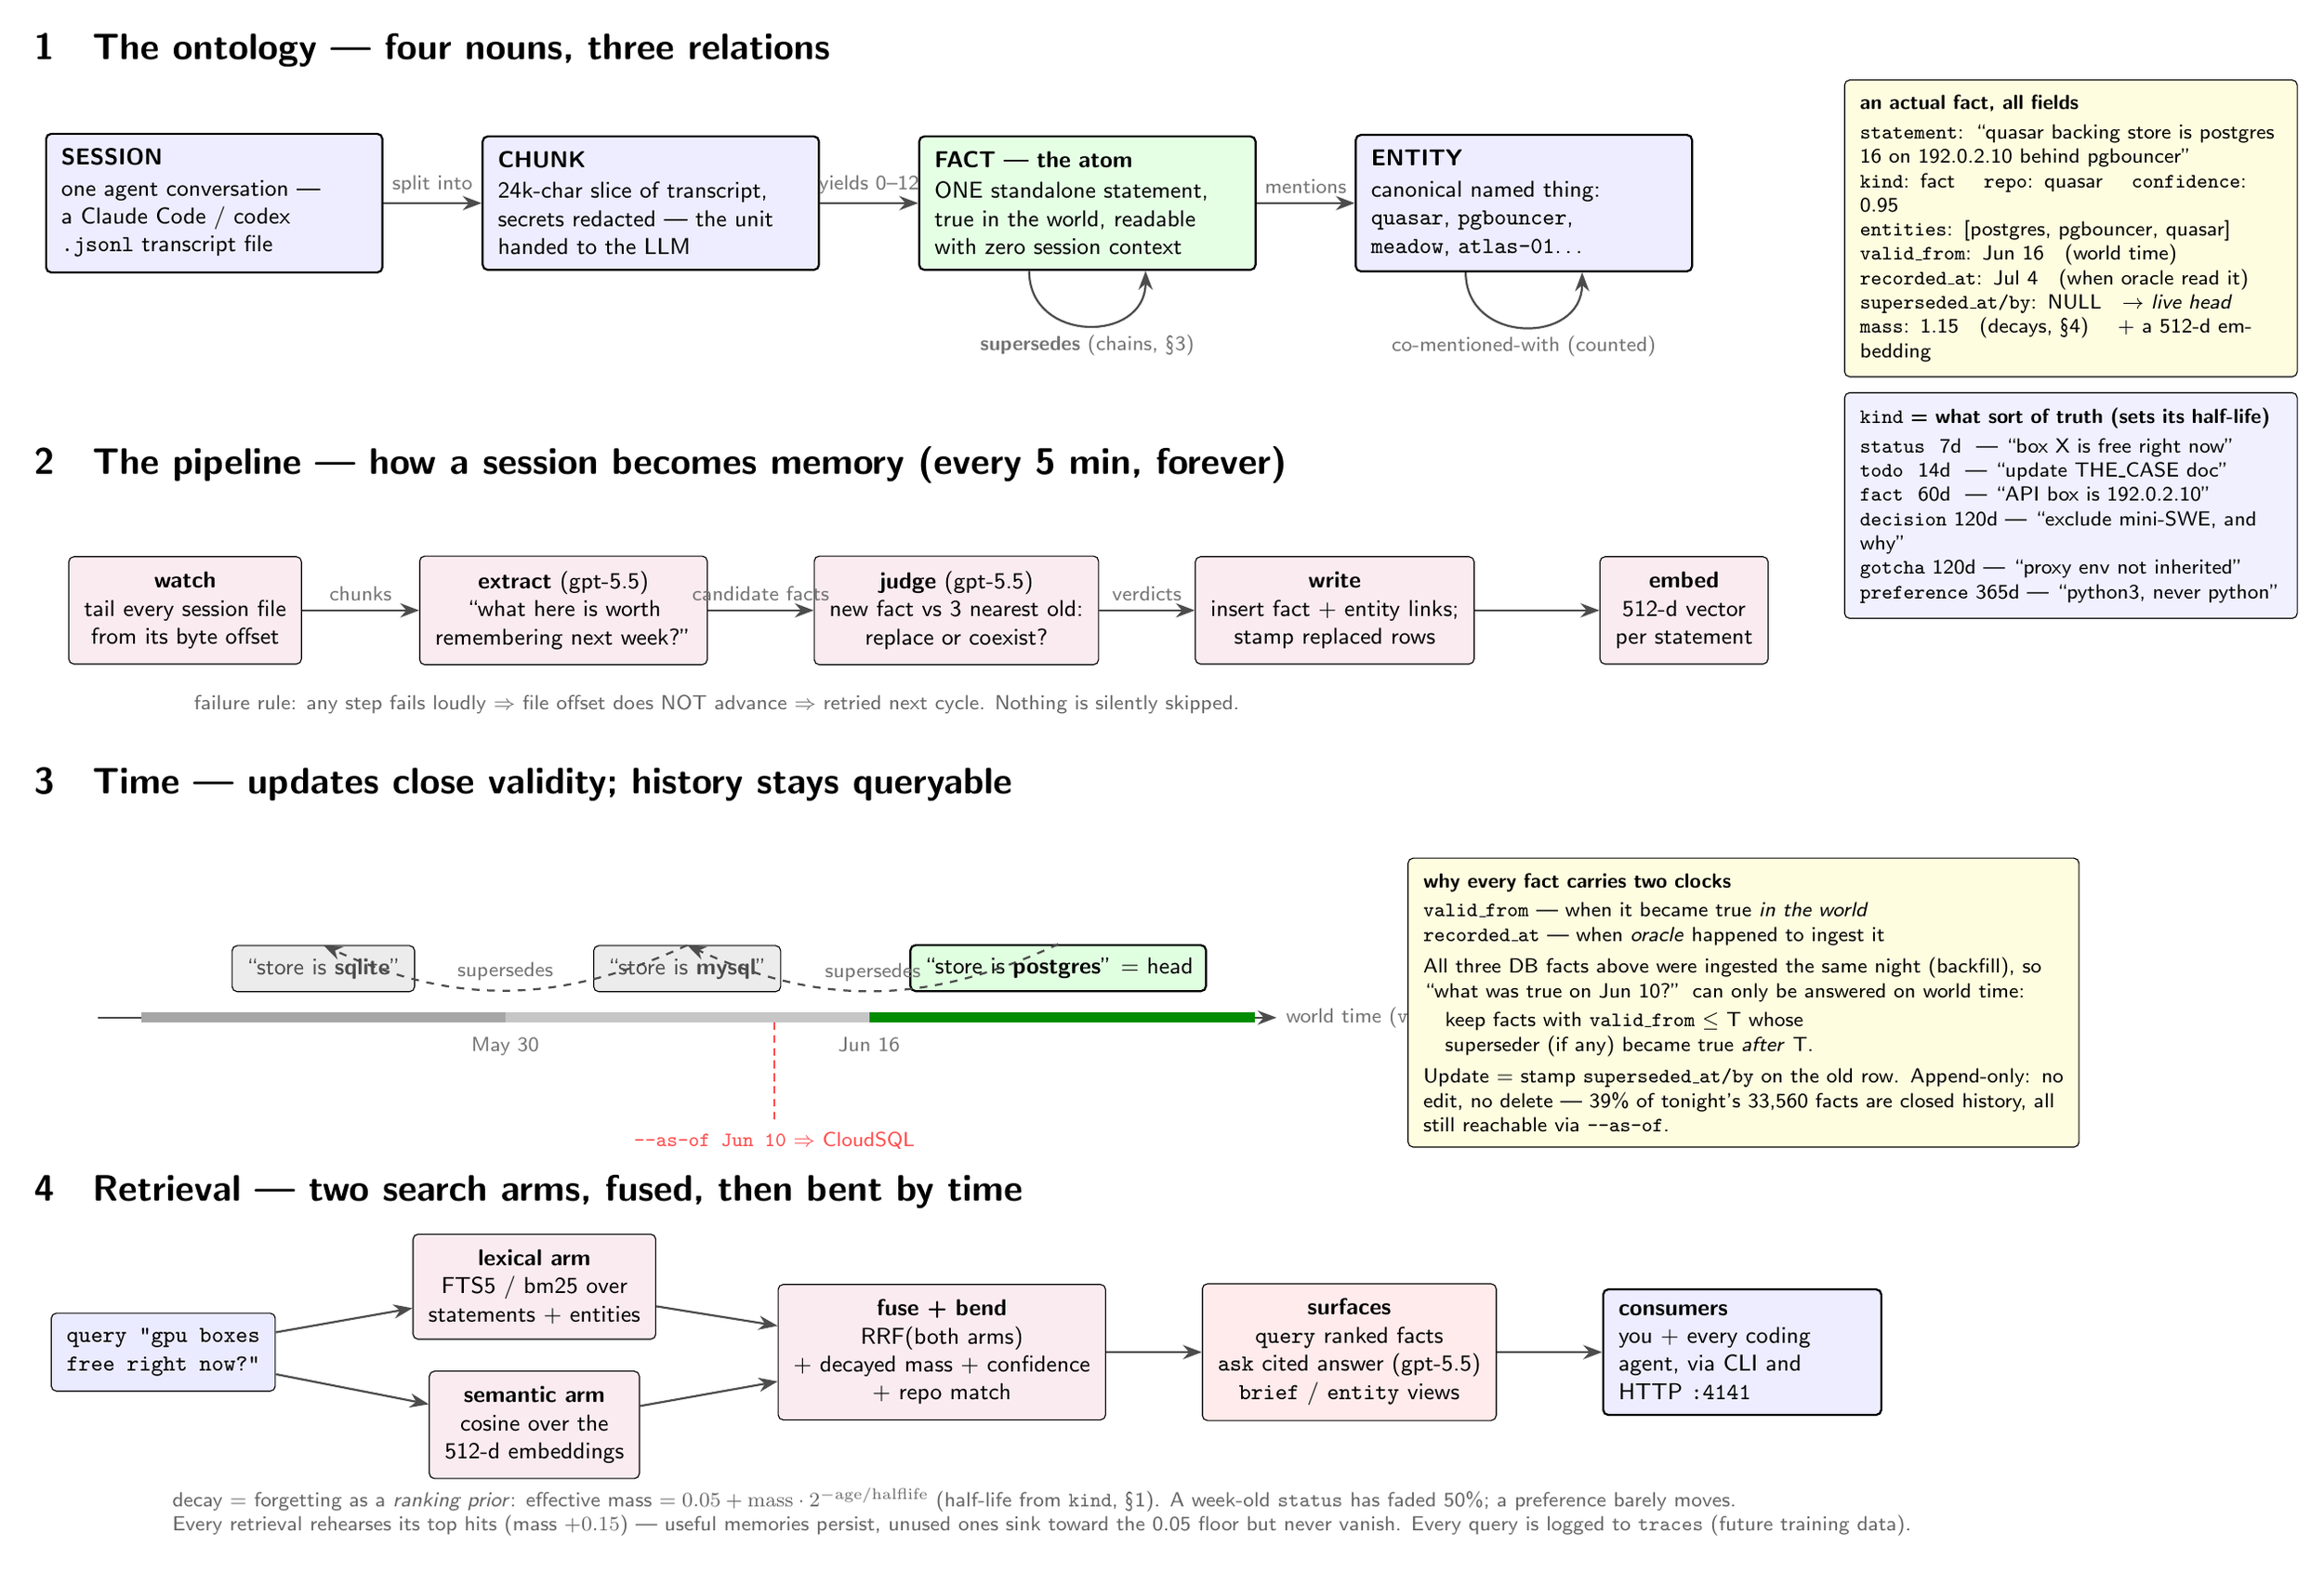
\begin{tikzpicture}[
  font=\sffamily\small,
  noun/.style={draw, thick, rounded corners=2pt, fill=blue!7, inner sep=6pt, align=left, text width=42mm},
  card/.style={draw, rounded corners=2pt, fill=yellow!12, inner sep=6pt, align=left, font=\sffamily\footnotesize, text width=58mm},
  stp/.style={draw, rounded corners=2pt, fill=purple!8, inner sep=6pt, align=center},
  dead/.style={draw, rounded corners=2pt, fill=gray!15, text=black!70, inner sep=5pt, align=center},
  live/.style={draw, thick, rounded corners=2pt, fill=green!12, inner sep=5pt, align=center},
  lbl/.style={font=\sffamily\footnotesize, text=black!55},
  head/.style={font=\sffamily\Large\bfseries},
  sub/.style={font=\sffamily\footnotesize, text=black!60},
  arr/.style={-{Stealth[length=2.6mm]}, thick, black!70}
]

% =====================================================================
% ROW 1 — ONTOLOGY: the four nouns
% =====================================================================
\node[head, anchor=west] at (0,26.3) {1 \; The ontology --- four nouns, three relations};

\node[noun] (sess) at (2.6,24.2)
  {\textbf{SESSION}\\[1pt] one agent conversation ---\\ a Claude Code / codex\\ \texttt{.jsonl} transcript file};
\node[noun] (chunk) at (8.6,24.2)
  {\textbf{CHUNK}\\[1pt] 24k-char slice of transcript,\\ secrets redacted --- the unit\\ handed to the LLM};
\node[noun, fill=green!10] (fact) at (14.6,24.2)
  {\textbf{FACT --- the atom}\\[1pt] ONE standalone statement,\\ true in the world, readable\\ with zero session context};
\node[noun] (ent) at (20.6,24.2)
  {\textbf{ENTITY}\\[1pt] canonical named thing:\\ \texttt{quasar}, \texttt{pgbouncer},\\ \texttt{meadow}, \texttt{atlas-01}\ldots};

\draw[arr] (sess) -- node[lbl, above]{split into} (chunk);
\draw[arr] (chunk) -- node[lbl, above]{yields 0--12} (fact);
\draw[arr] (fact) -- node[lbl, above]{mentions} (ent);
% self relations
\draw[arr] (fact.south) ++(-8mm,0) to[out=-90,in=-90, looseness=1.6]
  node[lbl, below]{\textbf{supersedes} (chains, \S3)} ++(16mm,0);
\draw[arr] (ent.south) ++(-8mm,0) to[out=-90,in=-90, looseness=1.6]
  node[lbl, below]{co-mentioned-with (counted)} ++(16mm,0);

% the example fact card
\node[card, anchor=north west] (ex) at (25.0,25.9)
  {\textbf{an actual fact, all fields}\\[2pt]
   \texttt{statement}: ``quasar backing store is postgres 16 on 192.0.2.10 behind pgbouncer''\\
   \texttt{kind}: fact \quad \texttt{repo}: quasar \quad \texttt{confidence}: 0.95\\
   \texttt{entities}: [postgres, pgbouncer, quasar]\\
   \texttt{valid\_from}: Jun 16 \; (world time)\\
   \texttt{recorded\_at}: Jul 4 \; (when oracle read it)\\
   \texttt{superseded\_at/by}: NULL \; $\rightarrow$ \emph{live head}\\
   \texttt{mass}: 1.15 \; (decays, \S4) \quad + a 512-d embedding};

% kinds mini-table
\node[card, anchor=north west, fill=blue!6] (kinds) at (25.0,21.6)
  {\textbf{\texttt{kind} = what sort of truth (sets its half-life)}\\[2pt]
   \texttt{status}\ \ 7d \ --- ``box X is free right now''\\
   \texttt{todo}\ \ 14d \ --- ``update THE\_CASE doc''\\
   \texttt{fact}\ \ 60d \ --- ``API box is 192.0.2.10''\\
   \texttt{decision} 120d --- ``exclude mini-SWE, and why''\\
   \texttt{gotcha}\ 120d --- ``proxy env not inherited''\\
   \texttt{preference} 365d --- ``python3, never python''};

% =====================================================================
% ROW 2 — PIPELINE: the verbs
% =====================================================================
\node[head, anchor=west] at (0,20.6) {2 \; The pipeline --- how a session becomes memory (every 5 min, forever)};

\node[stp] (watch) at (2.2,18.6)  {\textbf{watch}\\ tail every session file\\ from its byte offset};
\node[stp] (extr)  at (7.4,18.6)  {\textbf{extract} (gpt-5.5)\\ ``what here is worth\\ remembering next week?''};
\node[stp] (jdg)   at (12.8,18.6) {\textbf{judge} (gpt-5.5)\\ new fact vs 3 nearest old:\\ replace or coexist?};
\node[stp] (wrt)   at (18.0,18.6) {\textbf{write}\\ insert fact + entity links;\\ stamp replaced rows};
\node[stp] (emb)   at (22.8,18.6) {\textbf{embed}\\ 512-d vector\\ per statement};
\draw[arr] (watch) -- node[lbl,above]{chunks} (extr);
\draw[arr] (extr) -- node[lbl,above]{candidate facts} (jdg);
\draw[arr] (jdg) -- node[lbl,above]{verdicts} (wrt);
\draw[arr] (wrt) -- (emb);
\node[sub, anchor=west] at (2.2,17.3)
  {failure rule: any step fails loudly $\Rightarrow$ file offset does NOT advance $\Rightarrow$ retried next cycle. Nothing is silently skipped.};

% =====================================================================
% ROW 3 — TIME: chains + two clocks
% =====================================================================
\node[head, anchor=west] at (0,16.2) {3 \; Time --- updates close validity; history stays queryable};

% chain on a world-time line
\draw[arr] (1.0,13.0) -- (17.2,13.0) node[right, lbl] {world time (\texttt{valid\_from})};
\draw[gray!70, line width=4pt]        (1.6,13.0) -- (6.6,13.0);
\draw[gray!45, line width=4pt]        (6.6,13.0) -- (11.6,13.0);
\draw[green!55!black, line width=4pt] (11.6,13.0) -- (16.9,13.0);
\node[dead, anchor=south] (t1) at (4.1,13.35)  {``store is \textbf{sqlite}''};
\node[dead, anchor=south] (t2) at (9.1,13.35)  {``store is \textbf{mysql}''};
\node[live, anchor=south] (t3) at (14.2,13.35) {``store is \textbf{postgres}'' = head};
\node[lbl, below] at (6.6,12.85) {May 30};
\node[lbl, below] at (11.6,12.85) {Jun 16};
\draw[arr, dashed] (t2.north) to[bend left=25] node[lbl, above]{supersedes} (t1.north);
\draw[arr, dashed] (t3.north) to[bend left=25] node[lbl, above]{supersedes} (t2.north);
% as-of cursor
\draw[red!70, thick, dash pattern=on 3pt off 2pt] (10.3,11.6) -- (10.3,12.95);
\node[lbl, text=red!70, anchor=north] at (10.3,11.55) {\texttt{--as-of Jun 10} $\Rightarrow$ CloudSQL};

% two clocks explainer
\node[card, anchor=north west, text width=88mm] at (19.0,15.2)
  {\textbf{why every fact carries two clocks}\\[2pt]
   \texttt{valid\_from} --- when it became true \emph{in the world}\\
   \texttt{recorded\_at} --- when \emph{oracle} happened to ingest it\\[3pt]
   All three DB facts above were ingested the same night (backfill), so
   ``what was true on Jun 10?'' can only be answered on world time:\\[2pt]
   \quad keep facts with \texttt{valid\_from} $\le$ T whose\\
   \quad superseder (if any) became true \emph{after} T.\\[3pt]
   Update = stamp \texttt{superseded\_at/by} on the old row. Append-only:
   no edit, no delete --- 39\% of tonight's 33{,}560 facts are closed history,
   all still reachable via \texttt{--as-of}.};

% =====================================================================
% ROW 4 — RETRIEVAL: decay + hybrid ranking + surfaces
% =====================================================================
\node[head, anchor=west] at (0,10.6) {4 \; Retrieval --- two search arms, fused, then bent by time};

\node[stp, fill=blue!8] (q) at (1.9,8.4) {\texttt{query "gpu boxes}\\ \texttt{free right now?"}};
\node[stp] (bm) at (7.0,9.3) {\textbf{lexical arm}\\ FTS5 / bm25 over\\ statements + entities};
\node[stp] (cs) at (7.0,7.4) {\textbf{semantic arm}\\ cosine over the\\ 512-d embeddings};
\node[stp] (rrf) at (12.6,8.4) {\textbf{fuse + bend}\\ RRF(both arms)\\ $+$ decayed mass $+$ confidence\\ $+$ repo match};
\node[stp, fill=red!8] (out) at (18.2,8.4) {\textbf{surfaces}\\ \texttt{query} ranked facts\\ \texttt{ask} cited answer (gpt-5.5)\\ \texttt{brief} / \texttt{entity} views};
\node[noun, text width=34mm] (agents) at (23.6,8.4) {\textbf{consumers}\\ you + every coding\\ agent, via CLI and\\ HTTP \texttt{:4141}};
\draw[arr] (q) -- (bm); \draw[arr] (q) -- (cs);
\draw[arr] (bm) -- (rrf); \draw[arr] (cs) -- (rrf);
\draw[arr] (rrf) -- (out); \draw[arr] (out) -- (agents);
\node[sub, anchor=west, align=left] at (1.9,6.2)
  {decay = forgetting as a \emph{ranking prior}: effective mass $=0.05+\mathrm{mass}\cdot 2^{-\mathrm{age}/\mathrm{halflife}}$ (half-life from \texttt{kind}, \S1).
   A week-old \texttt{status} has faded 50\%; a preference barely moves.\\
   Every retrieval rehearses its top hits (mass $+0.15$) --- useful memories persist, unused ones sink toward the 0.05 floor but never vanish.
   Every query is logged to \texttt{traces} (future training data).};

\end{tikzpicture}
\end{document}
